\chapter{Attack Model}\label{ch:attack}

In this chapter, we will extensively present the threat model of BREACH. We will
explain the conditions that should be met so as to launch the attack and
describe our code implementation for that case. Also, we will investigate the
types of vulnerabilities in web applications that can be exploited with this
attack, as well as introduce alternative secrets, that have not been taken into
consideration before.

\section{Mode of Operation}\label{sec:mo}

\subsection{Description}

The first step of the attack is for the attacker to gain control of the victim's
network, specifically being aple to view the victim's encrypted traffic. This
can be accomplished using the Man-in-the-Middle techniques described in Section
\ref{sec:mitm}.

After that the BREACH JavaScript that issues the requests needs to be executed
from the victim's browser. The first way to do this is to persuade the victim to
visit a website where the script runs, usually with social engineering methods,
such as phishing or spam email.

The script issues multiple requests to the target endpoint, which are sniffed by
the attacker. As described in Section \ref{sec:sameorigin} the attacker cannot
read the plaintext response, however the length of both the request and the
response is visible on the network.

Each request contains some data, that is reflected in the response. Since the
victim is logged in the target endpoint website, the response body will also
contain the secrets. If the conditions defined in Section \ref{subsec:lz77} are
met, the secret and the reflected attacker input will be compressed and
encrypted.

By issuing a large amount of requests for different inputs, the attacker can
analyze the response lengths and extract information about the plaintext
secrets, as described above.

\subsection{Attack persistence}\label{sec:persistence}

In this section we will propose a \texttt{command-and-control} mechanism that
makes the attack much more practical. Specifically, we will describe how the
attack can be implemented even if the victim does not visit a contaminated web
page, but simply browses the HTTP web.

Since the attacker controls the victim's traffic, it is possible to inject the
attack script in a response from a regular HTTP website. The script will then
run on the victim's browser, as if the script was part of the page all along.

The following figure depicts this methodology, which is based on the fact that
regular HTTP traffic is not encrypted and also does not ensure data integrity.

\begin{figure}[H] \caption{Command-and-control mechanism.} \centering
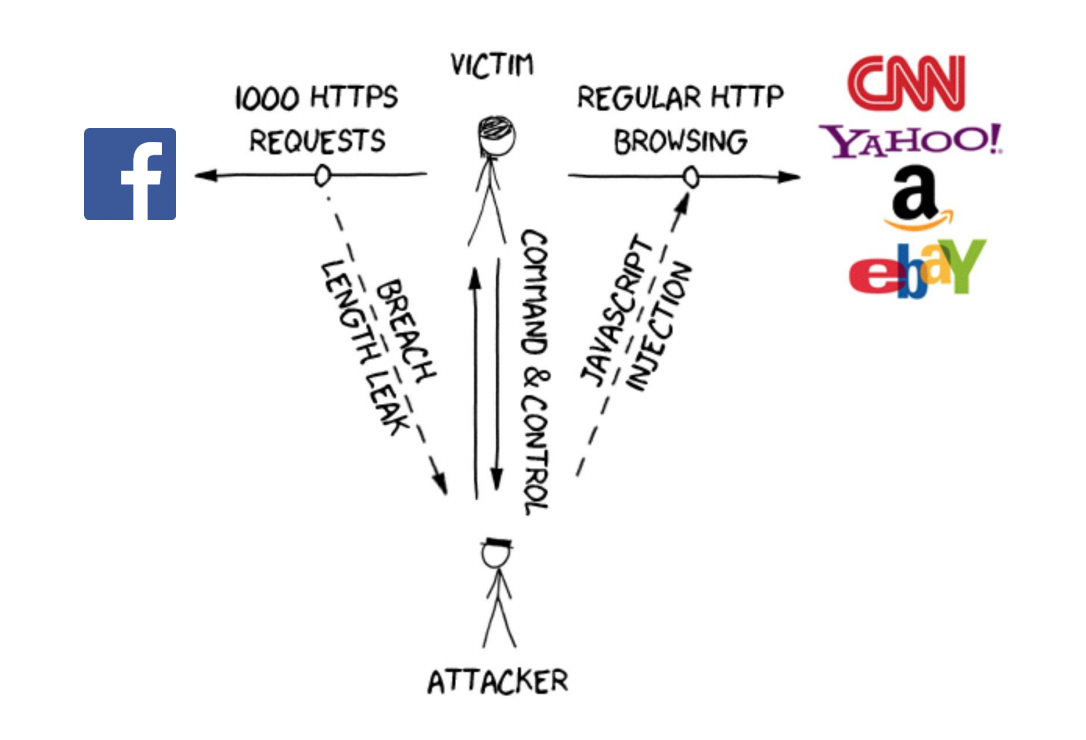
\includegraphics[width=0.6\textwidth]{diagrams/breach_mitm.png}\end{figure}

It is clear that, even if the victim breaks the connection, the script can be
injected in the next HTTP website that is requested, resuming the session from
where it was stopped.

\subsection{Man-in-the-Middle implementation}

In order to gain control of the victim's traffic towards a chosen endpoint, we
created a Python script that performs a Man-in-the-Middle. For the purpose of
this paper, the 'hosts' file of the test machine was configured to redirect
traffic regarding the chosen endpoint towards localhost, as shown below:

\plaintext{Test machine's hosts file}{hosts}

The user can set the IPs and ports of the victim and the endpoint, in order for
the Python script to open TCP sockets on both directions, so that traffic from
the victim to the endpoint and vice versa is routed through the
Man-in-the-Middle proxy.

After the environment is set, the script performs an infinite loop, where the
'select' module of Python is used to block the script until a packet is received
on either of the sockets.

When a packet is received, the source of the packet is identified and the data
is parsed in order to log the TLS header and the payload. After the information
needed is extracted, the packet is forwarded to the appropriate destination.

The parser is vital, since the header contains information regarding the version
of TLS used, as well as the length of the packet. For that purpose, we have
created a mechanism to perform packet defragmentation, since a TLS record can
span over multiple TCP packets. Specifically, the length of the packet payload
is compared to the length defined in the TLS header. In case the packet does not
contain all of the data declared, the number remaining of bytes is stored, so
that these bytes can be distinguished from the following packets of same origin.
In case the TLS header is fragmented, which can be deduced when the total bytes
of the packet, fragments from previous records excluded, are less than 5 bytes,
the actual data fragment needs to be stored, so that combined with the packets
to come it can translate to a valid TLS record information.

Finally, a TLS downgrade attack mechanism is also implemented. In case the user
wants to test whether a TLS downgrade is feasible, the Client Hello packet is
intercepted and dropped, while the MitM sends as a response a fatal 'HANDSHAKE
FAILURE' alert to the victim. The victim's browser is usually configured to
attempt a connection with a lower TLS version, where it should also include the
"TLS\_FALLBACK\_SCSV" option in the cipher suite list. If the server is
configured properly, the downgrade attempt should be recognised through the
"TLS\_FALLBACK\_SCSV" and the connection should be dropped. In other case, the
TLS version could be downgraded to a point where a less safe connection is
established, such as with version SSL 3.0 or using the RC4 stream cipher. For
further information on the downgrade vulnerability see POODLE \cite{poodle}.

The code of the Man-in-the-Middle proxy, as well as the constants library, can
be found in Appendix Sections \ref{sec:connect_py} and \ref{sec:constants_py}
respectively.

\subsection{BREACH JavaScript implementation}

For the implementation of the BREACH JavaScript, we assume the user has provided
the alphabet that the secret character belongs to, as well as the known prefix
needed to bootstrap the attack. This information will be written to a file used
by the JavaScript to perform the attack, an example of which is shown below:

\plaintext{File with request parameters.}{serial_request.txt}

The script then uses the jQuery library
\footnote{\url{http://code.jquery.com/jquery-2.1.4.min.js}} to read the info
from the file and begin the attack. If the file is corrupted or either of the
attack variables has changed, a delay of 10 seconds is introduced, so that the
system gets balanced. After that, a request for each item of the attack vector
is issued serially, continuing from the beginning when the end of the vector is
reached.

A delay of 10 seconds is also introduced if the above function fails for any
reason, i.e. if the info file does not exist. That way the attack is persistent
and it is the framework's responsibility to provide the JavaScript with a valid
information file.

For the purpose of this paper, the script was included in a local minimal HTML
web page that was visited in order for the attack to begin. However, with slight
modifications, it could be run on real world applications or injected in HTTP
responses, as described above.

The BREACH script and the HTML web page can be found in the Appendix Sections
\ref{sec:evil_js} and \ref{sec:index_html}.

\section{Vulnerable endpoints}\label{sec:vulnerabilities}

In the original BREACH paper \cite{breach}, Gluck, Harris and Prado investigated
the use of CSRF tokens included in HTTP responses as secrets to be stolen with
the attack. In this paper we suggest alternative secrets, as well as point out
specific vulnerabilities on widely used web applications, such as Facebook and
Gmail.

\subsection{Facebook Chat messages}\label{subsec:fb}

Facebook is the biggest social network as of 2015, with millions of people using
its chat functionality to communicate. Its mobile version, Facebook Touch
\footnote{\url{https://touch.facebook.com}} provides a lightweight alternative
for faster browsing. In this paper we will present a vulnerability that allows
    an attacker to steal chat messages from Facebook Touch, using BREACH attack.

Mobile versions of websites provide a good alternative compared to full versions
for a list of reasons. Firstly, these endpoints provide limited noise, given
    that they provide a lighter User Interface compared to full versions. As
    noise we could define any kind of string that changes between requests, such
    as timestamps or tokens, which can affect the length of the compressed HTML
    code for the same request. Secondly, given that the plaintext is smaller in
    mobile versions, the possibility of the text that lies between the secret
    and the reflection to be above the window of LZ77 compression is reduced.

Facebook has launched a mechanism to prevent the original BREACH attack against
CSRF tokens
\footnote{\url{https://www.facebook.com/notes/protect-the-graph/preventing-a-breach-attack/1455331811373632?_rdr=p}}.
However, as of August 2015, it has not created a mitigation technique against
the same attack on private messages. Such an attack vector is described in the
following paragraphs.

Facebook Touch provides a search functionality via URL, regarding chat messages
and friends. Specifically, when a request is made for
\url{https://touch.facebook.com/messages?q=}<search\_string>, the response
contains the chat search results for the given search string. If no match is
found, the response contains an empty search result page. However, this page
also contains the last message of the 5 latest conversations, which are
contained in the top drop-down message button of the Facebook User Interface, as
shown below:

\begin{figure}[H] \caption{Facebook Chat drop-down list.} \centering
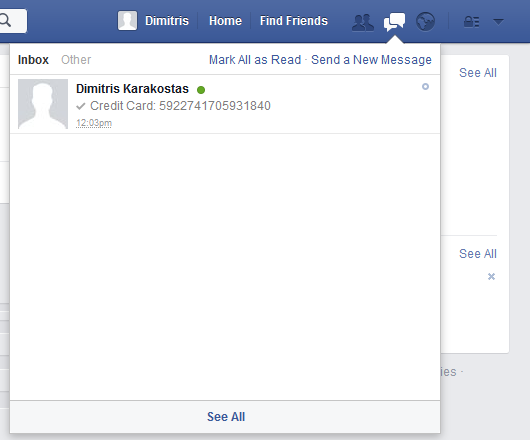
\includegraphics[width=0.6\textwidth]{diagrams/fb_message.png}\end{figure}

For the purpose of this paper we have created a lab account, that has no friends
and no user activity of any kind, except of a self-sent private message that
will be the secret to be stolen. That way the noise of a real-world account,
such as new messages or notifications, is contained to avoid the problems
described above.

The next step is to validate that the search string is reflected in the
response, which should also contain the private secret. Below is a fragment of
the HTML response body, where it can be clearly seen that this condition is met:

\begin{figure}[H] \caption{Facebook response body containing both secret and
reflection.} \centering
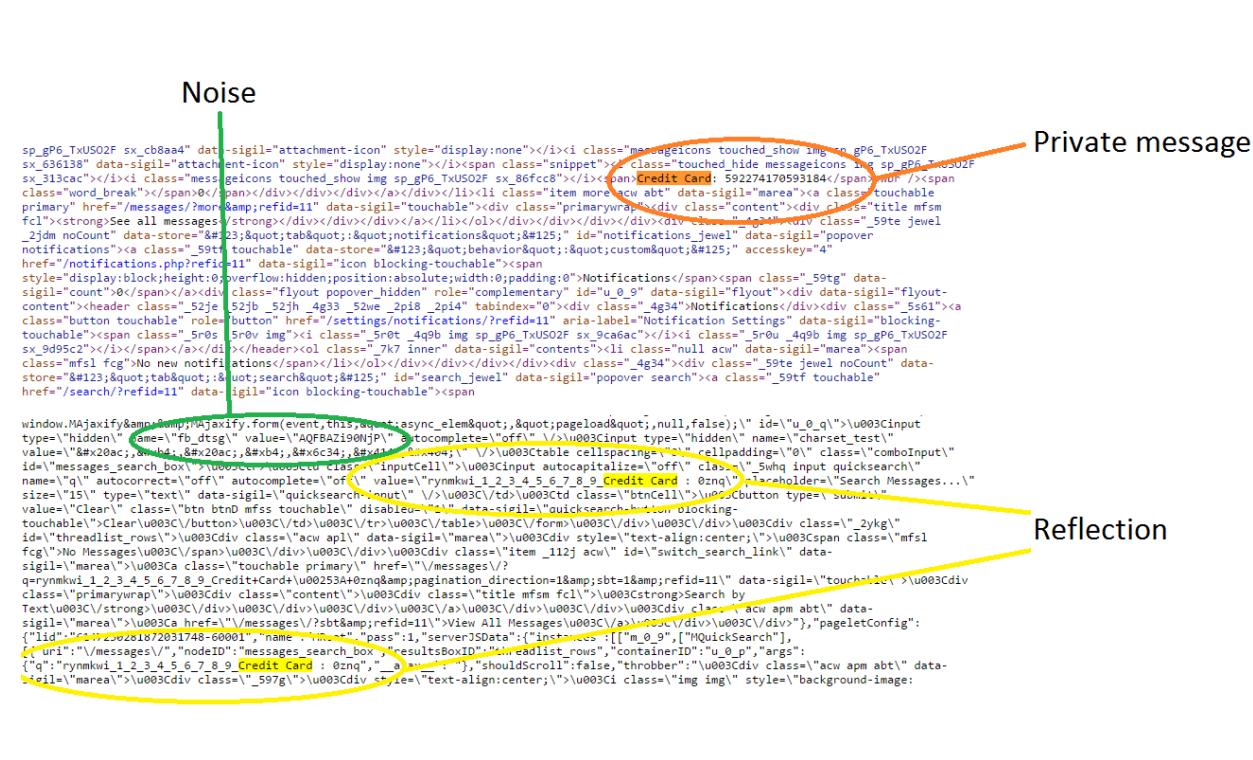
\includegraphics[width=1.1\textwidth]{diagrams/fb_response.png}\end{figure}

At this point, one of the basic assumptions of the attack, the fact that a
secret and an attacker input string should both be contained in the response,
has been confirmed, thus providing a vulnerability that can be exploited in the
context of the attack.

\subsection{Gmail Authentication token}

Gmail is one of the most used and trusted mail clients as of 2015. It also
provides a plain HTML version for faster, lightweight interaction
\footnote{\url{https://m.gmail.com}}. Gmail uses an authentication token, which
is a random string generated every time the user logs in the account.

In contrary to Facebook, Google has not issued any mechanism to mask the
authentication token for different sessions, but instead uses the same token for
a large amount of requests. This functionality could possibly result to a threat
against the confidentiality of the account, as will be described in the
following paragraphs.

Requests on \url{m.gmail.com} redirect to a route of the full website with an
additional parameter, specifically
\url{https://mail.google.com/mail/u/0/x/}<random\_string>, where the random
string is generated for every request on the website and can be used only for
the particular session.

Gmail also provides a search via URL functionality, similar to the one described
for Touch Facebook. Specifically, a user can search for mails using a URL like
    \url{https://mail.google.com/mail/u/0/x/?s=q&q=}<search\_string>. If no
    valid string is provided, where the random string is supposed to be, Google
    will redirect the request to a URL where the vacation with a randomly
    generated string and return an empty result page, stating the search action
    as incomplete, as shown below:

\begin{figure}[H] \caption{Invalid Gmail search.} \centering
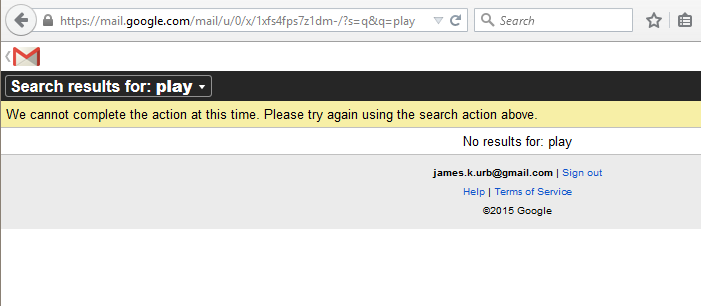
\includegraphics[width=1\textwidth]{diagrams/gmail_search.png}\end{figure}

However, the HTML body of the response contains both the search string and the
authentication token, as can be seen in the following figure:

\begin{figure}[H] \caption{Gmail response body containing both secret and
reflection.} \centering
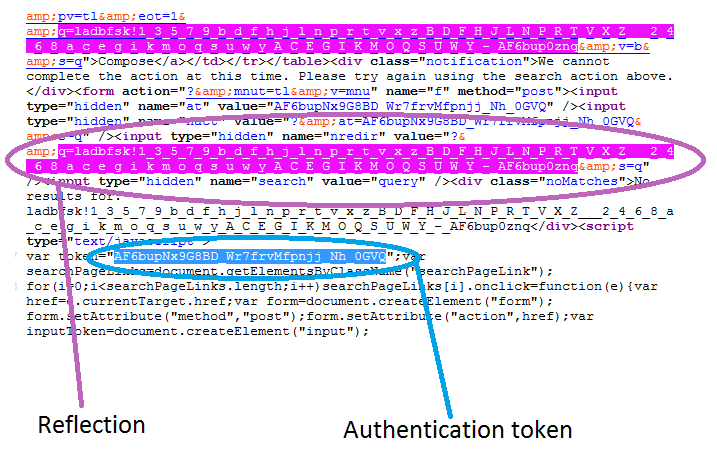
\includegraphics[width=1\textwidth]{diagrams/gmail_response.png}\end{figure}

Another vulnerability can be exploited when trying to find the first three
characters to bootstrap the attack. In the response body, the authentication
token is included as below:

\begin{figure}[H] \caption{Gmail authentication token.} \centering
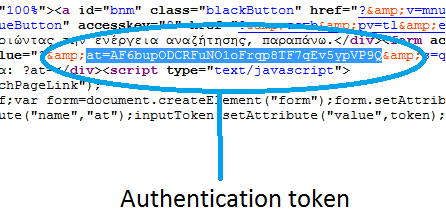
\includegraphics[width=0.6\textwidth]{diagrams/gmail_bootstrap.png}\end{figure}

The authentication token is preceded by the characters "at=", which can be used
at the beginning of the attack. Furthermore, the prefix "AF6bup" of the token is
static, regardless of the session and the account used. This prefix can also be
used in a similar manner to bootstrap the attack.

\subsection{Gmail private emails}

Another opportunity for the attack is provided by the search functionality of
the full Gmail website. If a user issues a search request in a URL as
\url{https://mail.google.com/mail/u/0#search/}<search\_string> and the search
response is empty, the HTML body will also contain both the Subject and an
initial fragment of the body of the latest inbox mails, as shown below:

\begin{figure}[H] \caption{Gmail empty search response containing latest mails.}
\centering
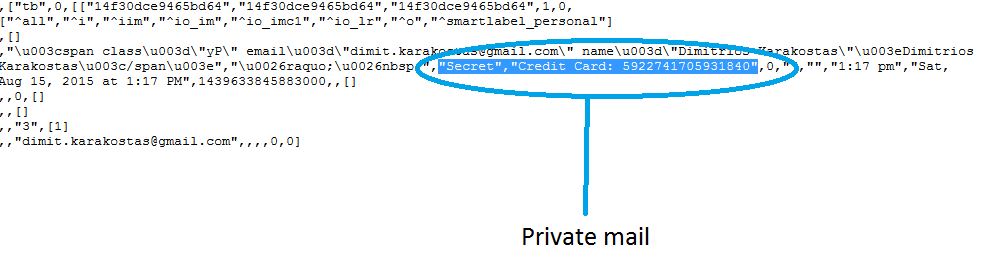
\includegraphics[width=1.1\textwidth]{diagrams/gmail_plain_response.png}\end{figure}

Although in that case, the response body does not include the search string, an
attacker could send multiple mails to the victim, which would be included in the
response as described. That way, the attacker could insert a chosen plaintext in
the HTML body and configure the attack under that context.

The above vulnerability shows that secrets and attacker input cannot always be
distinguished. In this case, both the secret and the input are emails, i.e. one
and the same, making the mitigation of the attack particularly hard.

\section{Validation of secret-reflection compression}\label{sec:mitmproxy}

In previous sections, we have found multiple vulnerabilities on known websites.
We have confirmed that the attacker's chosen plaintext and the secret are both
contained in the HTML response body. In this section, we will present a
methodology to confirm that the chosen plaintext and the secret are compressed
well, when the plaintext matches the secret, and badly in any other case.

The first tool used is mitmproxy \footnote{\url{https://mitmproxy.org}}.
Mitmproxy is described as "an interactive console program that allows traffic
flows to be intercepted, inspected, modified and replayed". For the purposes of
our work, mitmproxy was used to extract the compressed HTML body of two search
request, in the Facebook context described in Section \ref{subsec:fb}. The first
search string contained a selected prefix followed by an incorrect character,
while the second contained the same prefix followed by the correct character of
    the secret.

The second tool used is infgen \footnote{\url{http://www.zlib.net/infgen.c.gz}}.
Infgen is a disassembler that gets a gzip as an input and outputs the huffman
tables and the LZ77 compression of the initial data stream.

Applying infgen on the two HTML responses we obtained with mitmproxy, the
comparison regarding the correct and the incorrect search string can be seen in
the following figure:

\begin{figure}[H] \caption{Comparison of two compressed responses.}
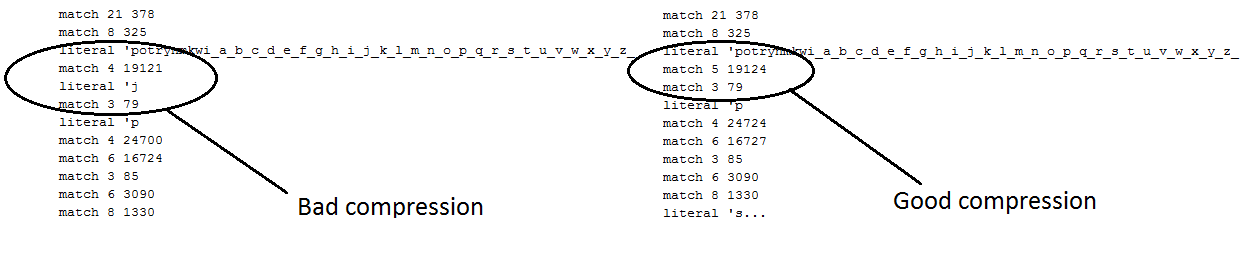
\includegraphics[width=1.15\textwidth]{diagrams/compression_comparison.png}\end{figure}

The left part of the figure shows the compression when the incorrect character
is used. In that case, the prefix is matched, therefore 4 characters are
compressed, however the next character is not compressed and is included as a
literal instead.

The right part shows the correct character compression, in which case both the
prefix and the character are compressed, resulting in 5 total characters to be
included in the reference statement and no literal statement.

It is understood that, in the second case, since the compression is better, the
LZ77 compressed text is smaller, possibly resulting to the final encrypted text
to be smaller.

The above described methodology can be used in any case, in order to test
whether a website compresses two portions of text and to verify that the
conditions of a PCPA attack are met.
